\section{Cache adaptatif} % (fold)
\label{sec:cache_adaptatif}

\begin{frame}{Contribution}
  \begin{figure}
    \centering
    %   \documentclass[crop,tikz]{standalone}% 'crop' is the default for v1.0, before it was 'preview'
% %\usetikzlibrary{...}% tikz package already loaded by 'tikz' option
% \usepackage[utf8]{inputenc}

% \usepackage{tikz}
% \usetikzlibrary{
%   arrows,
% automata,
% backgrounds,
% calc,
% decorations.pathreplacing,
% fit,
% petri,
% positioning,
% shadows,
% shapes,
% snakes,
% }


% % \begin{document}

  \begin{tikzpicture}%[scale = .8, every node/.style={scale = .8}]

%   % définition des styles
%   \tikzstyle{visible}=[draw, fill=blue!50]
%   \tikzstyle{hidden}=[ draw, fill=gray!20]
%   \tikzstyle{router}=[circle, draw, fill=orange!50,text=black]
%   \tikzstyle{child}=[circle, draw, fill=yellow!50,text=black]
%   \tikzstyle{root}=[circle, draw, fill=red!50,text=black]

  % les nœuds
  \node[draw, fill=red!50,] (rpca) {\begin{tabular}{c}Cache\\adaptatif\end{tabular}};
  \node[ left=of rpca] (queries) {\begin{tabular}{c}Requetes\\ applicatives\end{tabular}};
  \node[draw, below=of rpca] (setup) {\begin{tabular}{c}Setup\end{tabular}};
  \node[ right=of rpca] (QUERIES) {\begin{tabular}{c}Requetes\\ applicatives\end{tabular}};

%   \node[visible, below=of gw] (adapt) {Calcul des durées de validité optimales};


%   % Réseau contraint
%   \node[root] (1) at (-4, 0) {};
%   \node[router] (2) at (-5, 1) {};
%   \node[child] (3) at (-5, -1) {};
%   \node[child] (4) at (-6, 2) {};
%   \node[child] (5) at (-6, 0) {};

%   % \node[cloud, cloud puffs = 10, minimum width = 4cm, draw, fill = gray!10] (cloud) at (5,0) {Réseau local};
%   \node[draw] (cloud) at (5,0) {Réseau local};

%  \node [fit=(1) (2) (3) (4) (5), rounded corners, draw=black!50] (lln) {};
%  \node [below=.3 cm of lln] {LLN};

\path
  (setup) edge[->] (rpca)

  (QUERIES) edge[->, ultra thick] (rpca)
  (queries) edge[<-, ultra thick, dashed] (rpca)

%   % Réseau contraint
%   (gw) edge[<->, thick] node [above] {$r_u$} (1)
%   (1) edge[<->] (2)
%   (1) edge[<->] (3)
%   (2) edge[<->] (4)
%   (2) edge[<->] (5)

%   % Réseau conventionnel
%   (gw.east) edge[<->, ultra thick] node [above] {$T_u$} (cloud)

%   % Cache
%   (gw) edge[->,very thick, bend left=10] node [midway,right] {$(\mathcal{T}, \mathcal{L})$} (adapt)
%   (adapt) edge[->,very thick, bend left=10] node [left] {$\mathcal{C}$} (gw)
  ;

  \end{tikzpicture}
  % \end{document}
  \end{figure}

  \begin{alertblock}{Idée clé}
    Mettre en cache une réponse pour moins solliciter le réseau de capteurs.
  \end{alertblock}

\end{frame}

\begin{frame}{Architecture d'un proxy inverse}
  \begin{figure}
    \centering
    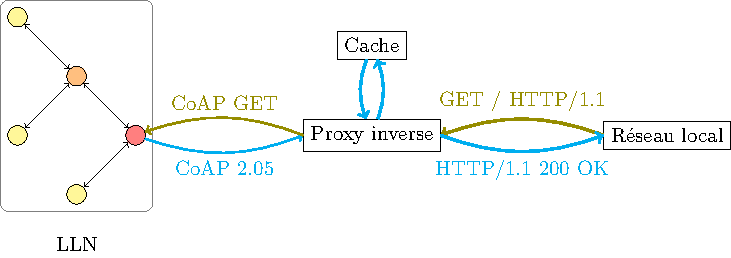
\includegraphics[width=0.8\textwidth]{figures/schema_rpc_slides.pdf}
  \end{figure}

  \begin{block}{Reverse Proxy Cache}
    \begin{itemize}
      \item Traduction de protocoles (Interopérabilité)
      \item Architecture client / serveur
      \item Intercepte les requêtes entrantes
      \item Chaque réponse a un temps de validité en cache
    \end{itemize}
    \end{block}
\end{frame}

\begin{frame}{Proxy inverse (miss)}
  \begin{figure}
    \centering
    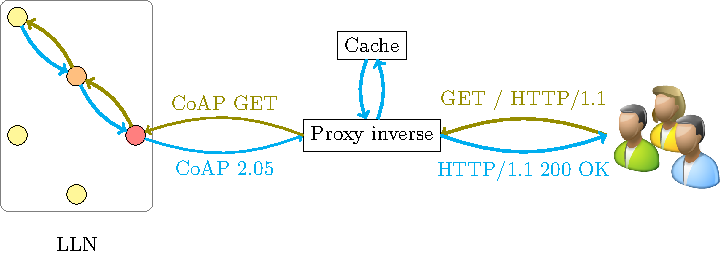
\includegraphics[width=\textwidth]{figures/schema_rpc_miss_slides.pdf}
  \end{figure}
\end{frame}

\begin{frame}{Proxy inverse (hit)}
  \begin{figure}
    \centering
    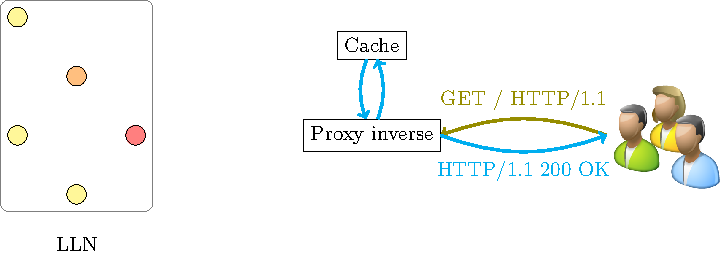
\includegraphics[width=\textwidth]{figures/schema_rpc_hit_slides.pdf}
  \end{figure}
\end{frame}

\begin{frame}\frametitle{Objectifs antagonistes}

  % \begin{block}{Contraintes}
  %   \begin{itemize}
  %     \item Les nœuds veulent répondre au moins de requêtes possibles
  %     \item Les utilisateurs veulent les réponses les plus récentes possibles
  %   \end{itemize}
  % \end{block}

  \begin{figure}
    \centering
    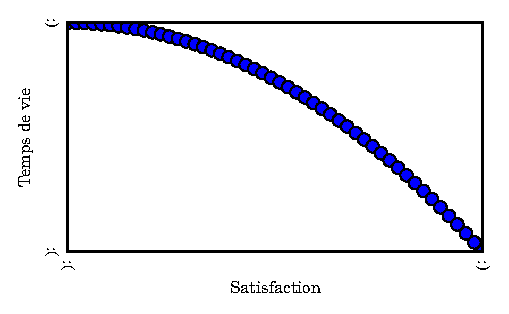
\includegraphics[width=\textwidth]{figures/schema_pareto.pdf}
  \end{figure}

  % \begin{alertblock}{Modèle de résolution}
  %   \begin{itemize}
  %     \item Utilisation d'algorithme génétique pour la résolution d'un problème multi-objectifs (Satisfaction ou Durée de vie)
  %     \item Front de Pareto $\to$ approximation des solutions optimales
  %     \item Fournir les temps de validité optimaux pour les réponses en cache par rapport à une dégradation de qualité de service donnée
  %   \end{itemize}
  % \end{alertblock}


  \begin{figure}
    
  \end{figure}

  \pnote{
    - L'algorithme génétique est généraliste il fonctionne quelque soit la définition des contraintes
  }
  \pnote{
    - Il repose sur un grand nombre de paramètre mais peut fonctionner efficacement avec une configuration par défaut.
  }
\end{frame}


\begin{frame}{Architecture du RPCA}
  % \begin{block}{Reverse proxy cache adaptatif}
  %    \begin{description}
  %      \item[$r_u$] Temps moyen entre requête entrant dans le LLN
  %      \item[$T_u$] Temps moyen entre requête venues des utilisateurs
  %      \item[$\mathcal{C}$] Ensemble des temps de validité en cache
  %      \item[$\mathcal{T}$] Topologie du LLN
  %      \item[$\mathcal{L}$] Objectif de durée de vie du LLN
  %    \end{description}
  % \end{block}

  \begin{figure}
    \centering
    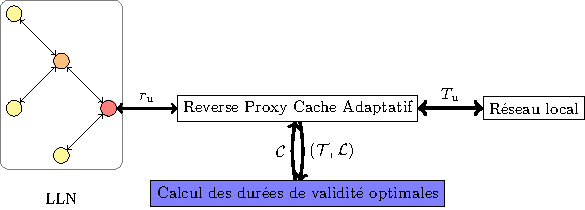
\includegraphics[width=.8\textwidth]{figures/schema_rpca_slides.pdf}
  \end{figure}

  \begin{block}{Principe du reverse Proxy Cache Adaptatif}
    $$(\mathcal{T}, \Gamma) \implies (\mathcal{C}, \mathcal{L})$$
  \end{block}

\end{frame}

\begin{frame}{Modèle de cache}
  \begin{block}{Hypothèses}
    \begin{description}
      \item[$c_u$] Temps de vie en cache d'une réponse
      % \item[$\lambda_u$] Constante du trafic de poisson vers $u$
      \item[$m_u$] Ratio de requête passantes vers les nœuds capteurs (miss ratio)
      % \item[$h_u$] Ratio de requête traitées par le cache (hit ratio)
    \end{description}
  \end{block}
  \begin{alertblock}{Modèle de cache}
    \begin{align}
      m_u &= \frac{1}{1 + \frac{c_u}{T_u}}
      \label{cache:eq:cache_miss}\\
      % h_u &= 1 - m_u = \frac{\lambda_u c_u}{1 + \lambda_u c_u}
      % \label{cache:eq:cache_hit}\\
      r_u &= \frac{T_u}{m_u} = T_u \left (1 + \frac{c_u}{T_u} \right) = T_u + c_u
    \end{align}
  \end{alertblock}
\end{frame}

\begin{frame}{Satisfaction}

\begin{block}{Notations}
  \begin{description}
    \item[Contraintes:] $c_{min}(u) \leq c_u \leq c_{max}(u)$
    \item[$\mathcal{C}_{min}$:] $\{c_{min}(u),  \forall u\}$
    \item[$\mathcal{C}_{max}$:] $\{c_{max}(u),  \forall u\}$
    % \item[Satisfaction utilisateur:] $\forall u, \gamma_u = \dfrac{\cmax(u) - c_u}{\cmax(u) - \cmin(u)}$
    % \item[$\Gamma$:] Moyenne de tous les $\gamma_u$
  \end{description}  
\end{block}

  % \begin{block}{Bonjour}

  \begin{block}{Modèle de satisfaction}
    \begin{align*}
      \Gamma &= f(\mathcal{C})\\
      avec: f(\mathcal{C}_{min}) &= 1\\
      f(\mathcal{C}_{max}) &= 0
    \end{align*}
    $f$ est linéaire afin de simplifier les calculs.    
  \end{block}

%   \end{block}

%   % \begin{figure}
%   %   \centering
%   %   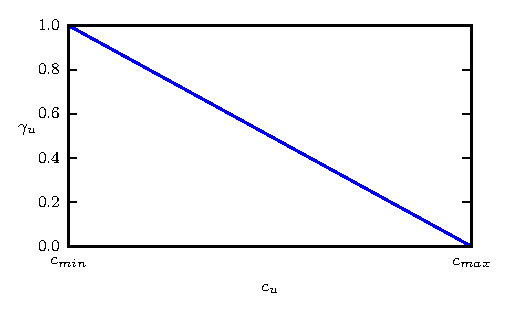
\includegraphics[width=.7\textwidth]{figures/satisfaction_utilisateur.pdf}
%   % \end{figure}

%   \pnote{
%     Une dégradation de service veut par exemple dire qu'on aura pas l'information la plus récente sur un emplacement de
%     parking.
%   }
\end{frame}

\begin{frame}{Modèle de durée de vie}
    % \begin{alertblock}{Énergie résiduelle}
    % \begin{align}

    %   E_r(T) &= E_0 - \int_0^T P(t) \mathrm{d}t\\
    %   % \int_0^T P(t) \mathrm{d}t &= \int_0^T P_{\sleep} \alpha_{\sleep}(t) \mathrm{d}t + \int_0^T P_{\listen} \alpha_{\listen}(t) \mathrm{d}t + \int_0^T P_{\tx} \alpha_{\tx}(t) \mathrm{d}t + \int_0^T P_{\rx} \alpha_{\rx}(t) \mathrm{d}t\\
      
    % \end{align}
    Énergie résiduelle = Énergie initiale - Énergie consommée
  % \end{alertblock}

  \begin{block}{Approximation de la puissance consommée}
    \begin{itemize}
      \item $P(t) = \alpha_{\sleep} P_{\sleep} + \alpha_{\listen} P_{\listen} + \alpha_{\tx} P_{\tx} + \alpha_{\rx} P_{\rx}$
      \item $P_{\sleep}, P_{\listen}, P_{\tx}, P_{\rx}$ connus.
      \item $\alpha_{\sleep}, \alpha_{\listen}, \alpha_{\tx}, \alpha_{\rx}$ à déterminer.
    \end{itemize}
  \end{block}

  \begin{block}{Cas}
    \begin{itemize}
      \item Serveur
      \item Routeur
    \end{itemize}
  \end{block}

\end{frame}


% \begin{frame}{Cas favorable}

%   \begin{block}{Transmission}
%     \begin{align}
%       T_{\pkt, \txtx} &= T_{\pkt}\\
%       T_{\pkt, \txrx} &= T_{\ack}
%     \end{align}
%   \end{block}

%   \begin{block}{Réception}
%     \begin{align}
%       T_{\pkt, \rxrx} &= T_{\pkt}\\
%       T_{\pkt, \rxtx} &= T_{\ack}
%     \end{align}
%   \end{block}

%   \pnote{
%     Ce cas correspond à un nœud qui transmet quand le récepteur s'allume et ne transmet donc qu'une seule fois son paquet.
%   }

%   \pnote{
%     - Le récepteur se réveille juste avant le début de l'émission et ne l'écoute donc qu'une seule fois $T_{\pkt, \rxrx} = T_\pkt$.
%   }

% \end{frame}

% \begin{frame}{Cas défavorable}
%   \begin{block}{Transmission}
%     \begin{align}
%       T_{\pkt, \txtx} &= T_{\pkt} + \left \lceil \frac{T_{\sleep}}{T_{\pkt} + T_{\detect}}\right\rceil T_{\pkt}\\
%       T_{\pkt, \txrx} &= \left \lceil \frac{T_{\sleep}}{T_{\pkt} + T_{\detect}}\right \rceil T_{\detect} + T_{\ack}
%     \end{align}
%   \end{block}

%   \begin{block}{Réception}
%     \begin{align}
%       T_{\pkt, \rxrx} &= 2T_{\pkt}\\
%       T_{\pkt, \rxtx} &= T_{\ack}
%     \end{align}
%   \end{block}

%   \pnote{
%     Le pire cas de transmission se produit quand le récepteur vient de s'endormir alors que le transmetteur veut commencer à envoyer sa trame.
%     Le transmetteur va envoyer la trame tous les $T_\pkt + T_\detect$ jusqu'à ce que le récepteur soit éveillé au début d'une transmission.
%     À chaque tentative, le transmetteur va écouter le canal pendant $T_\detect$ pour détecter un éventuel acquittement.
%     Ainsi il va effectuer $\lceil \frac{T_\sleep}{T_\pkt + T_\detect}\rceil$ transmissions sans succès puis quand le récepteur se réveille, il devra transmettre encore une fois pour que la trame soit  finalement reçue et acquittée.
%   }

%   \pnote{
%     - Le récepteur se réveille juste après le début de la transmission ainsi le nœud rate la première et doit en avoir une seconde pour recevoir correctement la trame. Ainsi dans le pire cas $T_{\pkt, \rxrx} = 2T_\pkt$.
%   }

% \end{frame}


\begin{frame}{Consommation des nœuds serveurs}

  \begin{figure}
    \centering
    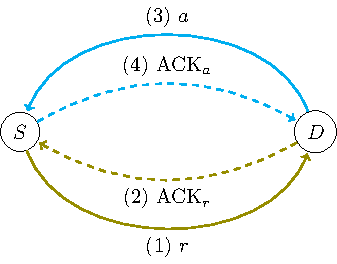
\includegraphics[scale=.8]{figures/conso_server_slides.pdf}
  \end{figure}


  % \begin{alertblock}{Consommation des nœuds serveurs}
    \begin{align}
      \alpha_{\server, \tx} &= \frac{T_{\req, \rxtx} + T_{\ans, \txtx}}{r_u}
      \label{contikimac:eq:coap_tx} \\
      \alpha_{\server, \rx} &= \frac{T_{\req, \rxrx} + T_{\ans, \txrx}}{r_u}
      \label{contikimac:eq:coap_rx}
    \end{align}
  % \end{alertblock}

\end{frame}

% \begin{frame}{Consommation des nœuds routeurs}
%   \begin{figure}
%     \centering
%     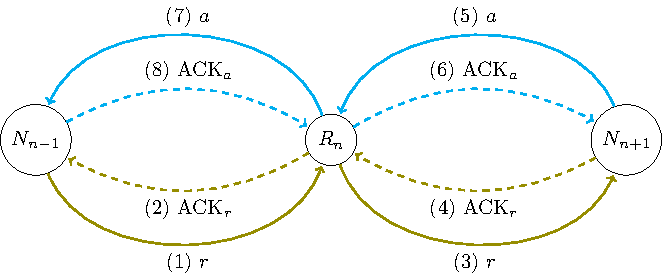
\includegraphics[scale=1]{figures/conso_routeur_slides.pdf}
%   \end{figure}
% \end{frame}

\begin{frame}{Consommation des nœuds routeurs}
  % \begin{block}{Charge pour les routeurs}
  %   \begin{align}
  %     T_{\router, \tx} &= T_{\req, \txtx} + T_{\req, \rxtx} + T_{\ans, \txtx} + T_{\ans, \rxtx}\\
  %     T_{\router, \rx} &= T_{\req, \rxrx} + T_{\req, \txrx} + T_{\ans, \rxrx} + T_{\ans, \txrx}
  %   \end{align}
  % \end{block}

  \begin{figure}
    \centering
    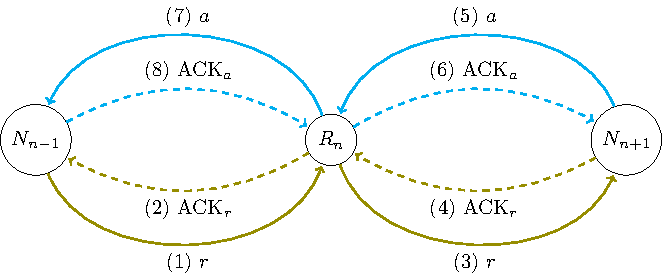
\includegraphics[scale=.8]{figures/conso_routeur_slides.pdf}
  \end{figure}

  % \begin{alertblock}{$\alpha_{\router, \tx}$ et $\alpha_{\router, \rx}$}
    \begin{align}
      \alpha_{\router, \tx} &= \sum_{j \in m_i} \frac{T_{\router, \tx, j}}{r_j}
      \label{contikimac:eq:router_tx}\\
      \alpha_{\router, \rx} &= \sum_{j \in m_i} \frac{T_{\router, \rx, j}}{r_j}
      \label{contikimac:eq:router_rx}
    \end{align}


  % \end{alertblock}
\end{frame}

\begin{frame}{Rappel sur le strobing (ContikiMAC)}
  \begin{figure}
    \centering
    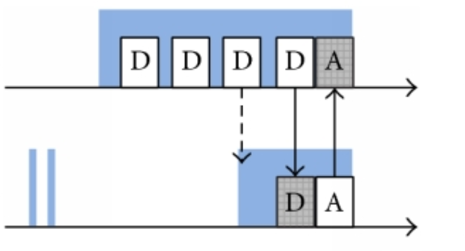
\includegraphics[width=0.8\textwidth]{figures/contikimac.png}
  \end{figure}
  \begin{block}{Notation}
    \begin{description}
      \item[$T_{\pkt}$] Temps pour émettre un paquet
      \item[$T_{\ack}$] Temps pour émettre un acquittement
      \item[$T_{\sleep}$] Temps de sommeil dans un cycle
      \item[$T_{\detect}$] Temps pour détecter l'arrivée d'un paquet d'acquittement
      % \item[$T_{\cycle}$] Temps d'un cycle complet
    \end{description}
  \end{block}
\end{frame}


% \begin{frame}{Cas moyen de $\alpha_{Tx}$ et $\alpha_{Rx}$}
\begin{frame}{Cas moyen}

    % Equiprobables + Linéaire $\implies$ moyenne = (meilleur + pire) / 2
    \begin{alertblock}{Transmission}
      Avec les paramètres du système $T_{\pkt}, T_{\sleep}, T_{\detect}, T_{\ack}$, on a :
    \begin{align*}
%       % T_{\pkt, \txtx} &= \dfrac{2 + \lceil \frac{T_\sleep - (T_\pkt + T_\detect)}{T_\pkt + T_\detect}\rceil}{2} T_\pkt
      T_{\pkt, \txtx} &=  \frac{T_{\pkt}}{2} \left\lceil \frac{T_{\sleep}}{T_{\pkt} + T_{\detect}}\right\rceil + T_{\pkt} \\
%       % T_{\pkt, \txrx} &= \dfrac{2 + \lceil \frac{T_\sleep - (T_\pkt + T_\detect)}{T_\pkt + T_\detect}\rceil}{2} T_\detect + T_\ack
      T_{\pkt, \txrx} &= \frac{T_{\detect}}{2} \left \lceil \dfrac{T_{\sleep}}{T_{\pkt} + T_{\detect}} \right \rceil + T_{\ack}
    \end{align*}
  \end{alertblock}

  \begin{alertblock}{Réception}
    \begin{align*}
      T_{\pkt, \rxrx} &= \frac{3 T_{\pkt}}{2} \mbox{\phantom{xxxxx}} T_{\pkt, \rxtx} = T_{\ack}
    \end{align*}
  \end{alertblock}

  \pnote{
    - Les deux cas sont équiprobables
  }
\end{frame}


\begin{frame}{Phases d'écoute et de sommeil}

  \begin{block}{Notation}
    \begin{description}
      % \item[$T_{\pkt}$] Temps pour émettre un paquet
      % \item[$T_{\ack}$] Temps pour émettre un acquittement
      % \item[$T_{\sleep}$] Temps de sommeil dans un cycle
      % \item[$T_{\detect}$] Temps pour détecter l'arrivée d'un paquet d'acquittement
      \item[$T_{\cycle}$] Temps d'un cycle complet
      \item[$T_{A}$] Temps actif
    \end{description}
  \end{block}


  \begin{alertblock}{Phase d'écoute}
    \begin{align}
      \alpha_{\listen} &= \frac{T_{\act}}{T_{\cycle}}(1 - \alpha_{\tx} - \alpha_{\rx})
    \end{align}
  \end{alertblock}
  \begin{alertblock}{Phase de sommeil}
    \begin{align}
      \alpha_{\sleep} &= \frac{T_{\cycle} - T_{\act}}{T_{\cycle}}(1 - \alpha_{\tx} - \alpha_{\rx})
    \end{align}
  \end{alertblock}

\end{frame}

\begin{frame}{Optimisation multi-objectifs}
  % \begin{columns}
  %     \begin{column}{0.48\textwidth}
  %       \begin{figure}
  %         % \centering
  %         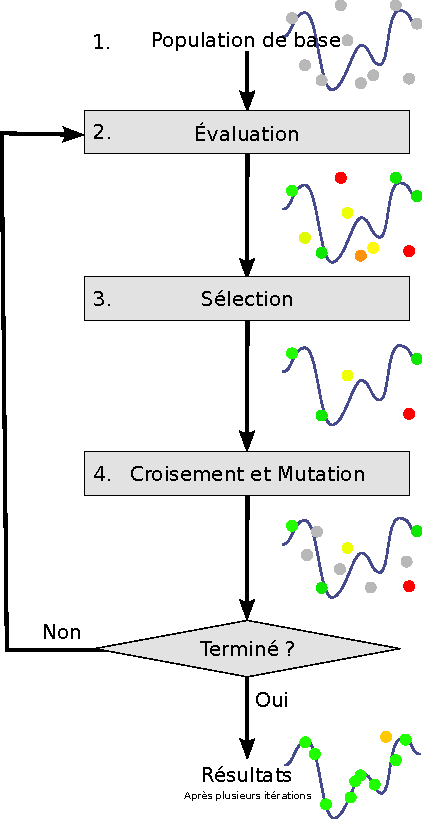
\includegraphics[scale=.5]{../img/algo_genetique.pdf}
  %       \end{figure}
  %     \end{column}
  %     \begin{column}{0.48\textwidth}
        \begin{alertblock}{Problème}
          \begin{itemize}
            \item f linéaire $\implies$ Résolution exacte
            \item f compliqué $\implies$ ?
          \end{itemize}
        \end{alertblock}
        \begin{alertblock}{Méta-heuristiques}
          \begin{itemize}
            \item Rapide
            \item Temps de calcul maîtrisé
            \item Hypothèses faibles
          \end{itemize}
        \end{alertblock}
        \begin{alertblock}{Algorithme génétique}
          \begin{itemize}
            \item Compatible avec multi-objectifs
            \item Population de solution (exploration des compromis)
            \item $\Gamma$ réglable sans recalculer
          \end{itemize}
        \end{alertblock}
  %     \end{column}
  % \end{columns}  

% Schéma à virer au besoin ?

\end{frame}

\begin{frame}{Validation expérimentale}
  \begin{figure}
    \centering
    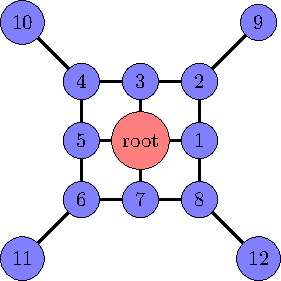
\includegraphics[scale=.7]{figures/topology_cache_slides.pdf}
  \end{figure}
  Repartition spatiale - Topologie arbitraire

  \begin{block}{Hypothèses}
    \begin{itemize}
      \item Trafic de Poisson stationnaire en entrée
      \item Résolution multi-objective exécutée puis déployée
      \item 50 requêtes par nœuds
      % \item Contiki / COOJA / Californium
    \end{itemize}
  \end{block}

  \pnote{
    - Nombre de requete traitée: 50
  }
  \pnote{
    - 10 runs par configuration pour les intervalles de confiance
  }
  \pnote{
    - 12 nœuds dans le réseau
  }
\end{frame}

\begin{frame}{Front de Pareto}

  \begin{figure}[tb]
    \centering
    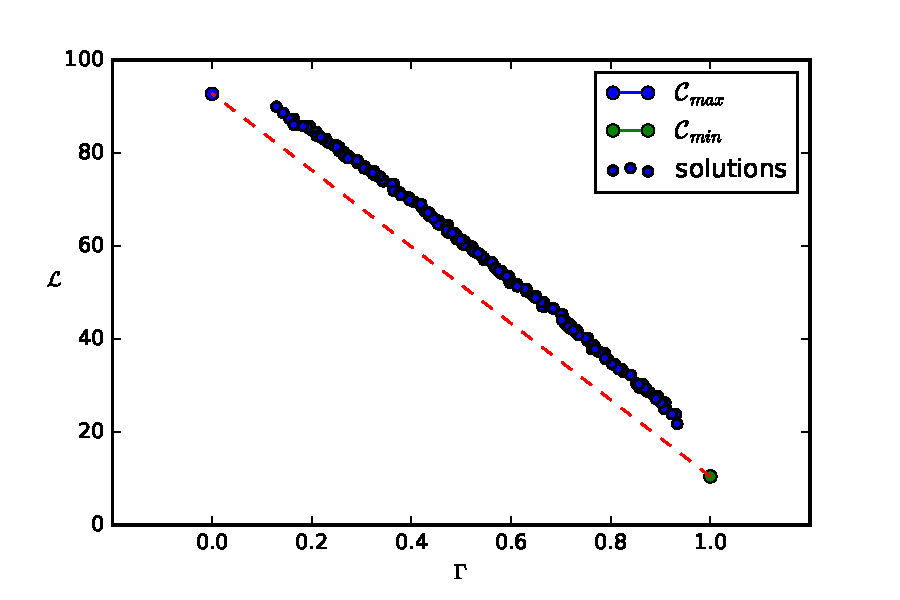
\includegraphics[width=0.75\textwidth]{../img/pareto.pdf}
  \end{figure}

  \begin{block}{Variables utilisées}
    \begin{description}
      \item[$\Gamma$] Satisfaction utilisateur moyenne
      \item[$\mathcal{L}$] Durée de vie du réseau (en jours)
    \end{description}
  \end{block}

  \pnote{
    - Chaque point solution est un C contenant l'ensemble des c_u.
  }
  \pnote{
    - Approximation du front de pareto
  }
  \pnote{
    - Les poins C_min et C_max => bornes
  }
  \pnote{
    - C_min garantie une fraîcheur aussi élevée que possible, mais raccourcit la durée de vie alors que
  }
  \pnote{
    - C_max garantie une durée de vie aussi longue que possible mais avec des fraicheur faibles.
  }
  \pnote{
    Une valeur haute de $c_u$ sera utilisée pour des nœuds ayant peu d'énergie.
  }
  \pnote{
    Par contre, une valeur $c_u$ petite sera pour des informations devant être aussi récentes que possible.
  }
\end{frame}


\begin{frame}{Exemple}

  \begin{figure}[tb]
    \centering
    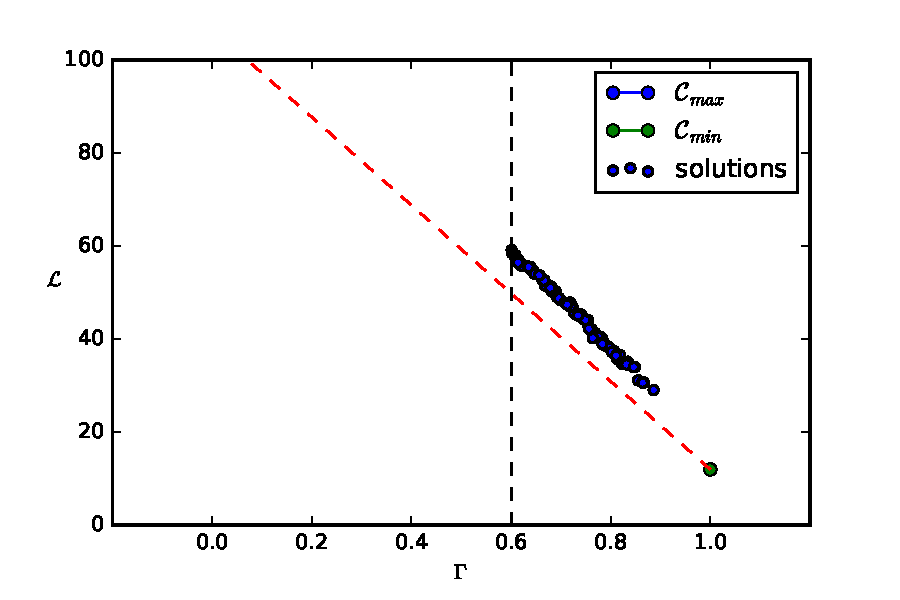
\includegraphics[width=0.75\textwidth]{figures/pareto_06.pdf}
  \end{figure}

  \begin{block}{Variables utilisées}
    \begin{description}
      \item[Dégradation de service moyenne tolérée:] $\Gamma > 0.6$
      \item[$\mathcal{L}$] Durée de vie du réseau maximale: 59 jours
    \end{description}
  \end{block}

\end{frame}


\begin{frame}{Cache hit ratio en fonction de $\lambda_u$ et $c_u$}

  \begin{figure}[ht]
    \centering
    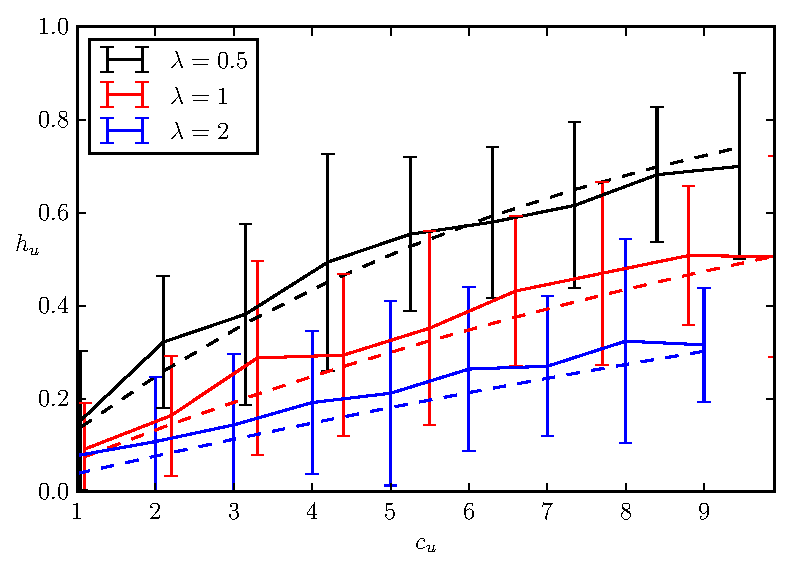
\includegraphics[width=.6\textwidth]{figures/new_cachinghit.pdf}
  \end{figure}

  \begin{block}{Variables utilisées}
    \begin{description}
      \item[$c_u$] Temps de validité en cache
      \item[$h_u$] Ratio de requêtes traitées par le cache (hit ratio)
      \item[$\lambda_u$] Rythme d'arrivée poissonien
    \end{description}
  \end{block}


  \pnote{
    - Tous les c_u et \lambda_u sont égaux entre eux (Simplification visuelle)
  }
  \pnote{
    - Plus $c_u$ est grand par rapport à $T_u = \frac{1}{\lambda_u}$, plus le cache est efficace, car la probabilité que la requête soit servie par le \ac{RPCA} augmente épargnant ainsi aux nœuds du \ac{LLN} de les traiter.
  }
  \pnote{
    - Quand $c_u$ est petit devant $T_u = \frac{1}{\lambda_u}$, la fréquence de requête est plus faible que le temps de vie dans le cache.
  Le cache est ici inefficace, car une réponse n'y vit pas assez longtemps pour être susceptible d'être utilisée.
  }
\end{frame}

\begin{frame}\frametitle{Durée de vie en fonction de $\lambda_u$ et $c_u$}

  \begin{figure}[ht]
    \centering
    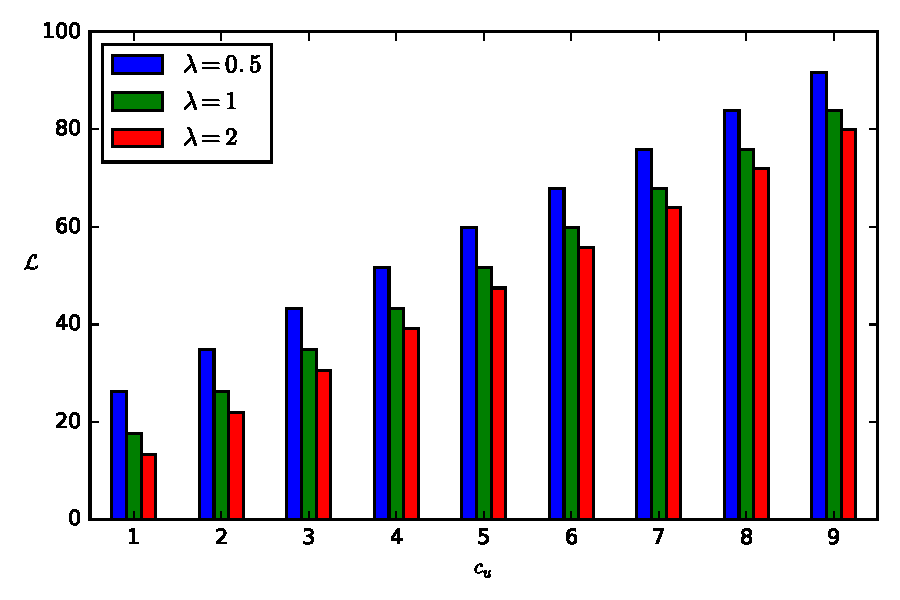
\includegraphics[width=0.7\textwidth]{figures/new_lifetime.pdf}
  \end{figure}

  \begin{block}{Remarques}
    \begin{itemize}
      \item Le réseau est considéré comme mort au premier nœud mort.
      \item Plus $c_u$ est élevé plus la durée de vie l'est aussi
    \end{itemize}
  \end{block}

\end{frame}
